
\documentclass[10pt]{article}

\usepackage{pgfplots}
\usepackage{tikz}
\usepackage{amsmath}
\usepackage{amssymb}     % for mathbb
\usepackage{enumerate}
\usepackage{xfrac}
\usepackage{float}
\usepackage{hyperref}
\usepackage{algorithmic}
\usepackage{algorithm}
\usepackage{booktabs}    % for beautiful tables
\usepackage{siunitx}     % for si units
\usepackage{color}
\usepackage{titlesec}    % for header spacing
\usepackage{caption}     % for caption*
\usepackage[capitalize]{cleveref}

\usepackage[backend=bibtex,style=ieee]{biblatex}

% set margins
\addtolength{\oddsidemargin}{-.875in}
\addtolength{\evensidemargin}{-.875in}
\addtolength{\textwidth}{1.75in}
\addtolength{\topmargin}{-.875in}
\addtolength{\textheight}{1.75in}

\setlength{\parindent}{0cm}        % no paragraph indentations
\setlength{\parskip}{0.5em}        % small paragraph spacing

\titlespacing\section{0pt}{10pt plus 4pt minus 2pt}{0pt plus 2pt minus 2pt}
\titlespacing\subsection{0pt}{10pt plus 4pt minus 2pt}{0pt plus 2pt minus 2pt}
\titlespacing\subsubsection{0pt}{10pt plus 4pt minus 2pt}{0pt plus 2pt minus 2pt}

\DeclareMathOperator*{\argmax}{arg\,max}

\newcommand{\calcium}[0]{Ca\textsuperscript{2+}}
\newcommand{\todo}[1]{\textcolor{red}{#1}}
\providecommand{\tw}[1]{{\tw[TIM: #1]}}

% monokai colors
\definecolor{color1}{RGB}{82,227,246}  % light blue
\definecolor{color2}{RGB}{167,243,113} % light green
\definecolor{color3}{RGB}{255,0,127}   % red
\definecolor{color4}{RGB}{249,151,31}  % orange
\definecolor{color5}{RGB}{121,171,255} % cobalt

\AtEveryBibitem{
\ifentrytype{inproceedings}{
    \clearlist{address}
    \clearlist{publisher}
    \clearname{editor}
    \clearlist{organization}
    \clearfield{url}  
    \clearfield{doi}  
    \clearfield{pages}  
    \clearlist{location}
 }{}
 }

\addbibresource{ref.bib}
\renewcommand*{\bibfont}{\footnotesize}

\begin{document}

\begin{center}
    {\LARGE Clustering of Neurons from Large-Scale Calcium Imaging Data}

    Stats 306b Project - Final Report

    Mohammad Ebrahimi and Tim Wheeler

    Spring 2015
\end{center}

\begin{abstract}
Fluorescent imaging allows for the analysis of signalling behavior on a per-neuron basis in anesthetized and awake behaving animals. % ~\cite{Mukamel2009}
Existing methods monitor {\calcium} dynamics over a large region, but recently developed automated methods allow for isolating signals and associating them with particular neurons.
The resulting set of candidate neurons suffers from the presence of background structures such as blood vessels.
This project applies clustering methods to candidate objects in a one-photon {\calcium} dataset for the classification of neurons from background structures.
\todo{Hierarchical clustering was performed to identify preliminary classes.}
\todo{Principle component analysis was performed to identify preliminary important features and a clustering analysis was conducted using the first two principle components.}
\todo{Sparse clustering and sparse principle component analysis were conducted to identify a reduced featureset which captures the majority of the variation in the data.}
\todo{Group validation was performed by comparing the clusters obtained in the first dataset to the clusters obtained in a withheld dataset.}
\todo{Results indicate...}
\end{abstract}


\section{Introduction}

\todo{Introduce away}

% One proposed method leverages spatio-temporal sparseness in elevated [\calcium] levels to identify neuronal spikes and associate them with particular regions in the source frames.
% The resulting work suffers from the presence of background structure such as blood vessels.
% This project aims to apply unsupervised learning methods to identify classes of identified objects from one-photon {\calcium} imaging in the primary visual cortex (V1) of awake behaving mice to aid in the automatic unsupervised classification of neurons from background structures.

\todo{Cover prior work}

\todo{Paper organization and results}


\section{Data Source}

Previous work by \citeauthor{Mukamel2009} obtained one-photon {\calcium} imaging recordings from the primary visual cortex of awake behaving mice.
Their work isolated candidate objects from cortex recordings of mice performing a go/no-go task for \num{30}-minute sessions over three consecutive days.
This work uses the isolated candidate objects, including frame images assocated with each of the extracted independent components and averaged signal traces associated with each candidate.

The complete cortex recording was segmented into a four-by-four grid.
Candidate object images are \num{500} $\times$ \num{500} pixel black and white frame averages that show the strength of their respective independent component over its corresponding segmented field of view. 
The pixel values correspond to the flourescent signal of the identified object, which may be a neuron, part of a blood vessel, or background noise.

Independent component traces were sampled at \num{6.7}\si{Hz}, totalling \num{1200} samples over each \num{30}-minute recording. The component traces of neurons possess indicative spikes with tapered decays corresponding to neuron activity, but also contain significant background noise.

Each recording contains a few thousand extracted objects, the idendity and quantity of which will vary between recordings.
The final feature set includes \num{5451} samples.
A previously conducted analysis of the dataset found that it contains approximately 50\% actual neurons~\todo{CITE?}.

\section{Features}

A set of \num{42} candidate features was extracted from the segmented image data and associated intracellular [\calcium] signals as is listed in~\cref{table:allfeatures}.
The set includes \emph{image features} obtained from the grayscale frame averages and \emph{trace features} from the independent component time series traces.

\begin{table}[h]
  \centering
  \small
  \caption{Candidate fatures extracted for each independent component in the {\calcium} imaging dataset}
  \label{table:allfeatures}
  \begin{tabular}{lll}
    \toprule
    \multicolumn{3}{c}{Image Features} \\
    \midrule

    area & pixels & peak region area  \\
    \addlinespace[2pt]
    perimeter & pixels & peak region perimeter \\
    \addlinespace[2pt]
    skew & - & peak region skew \\
    \addlinespace[2pt]
    peak & intensity &  maximum component intensity value  \\
    \addlinespace[2pt]
    roundness & - &  ratio proportional to area over squared perimeter\\
    \addlinespace[2pt]
    contrast & - &  contrast of normalized pixels in the component subregion \\
    \addlinespace[2pt]
    peak region mean & intensity &  mean intensity from pixels in peak region \\
    \addlinespace[2pt]
    peak region stdev & intensity\textsuperscript{2} & standard deviation of intensity from pixels in peak region \\
    \addlinespace[2pt]
    subregion mean & intensity &  mean intensity from pixels in component subregion \\
    \addlinespace[2pt]
    subregion stdev & intensity\textsuperscript{2} &  standard deviation of intensity from pixels in component subregion \\
    \addlinespace[2pt]
    primary directionality & - &  the directionality histogram bin of greatest value \\
    \addlinespace[2pt]
    directionality entropy & Hart &  the base-\num{10} entropy for the directionality histogram \\
    \midrule
    \multicolumn{3}{c}{Trace Features} \\
    \midrule

    \todo{trace 1} & \todo{???} &  \todo{a trace feature} \\
    \addlinespace[2pt]
    \todo{trace 2} & \todo{???} &  \todo{a trace feature} \\
    \addlinespace[2pt]
    \todo{trace 3} & \todo{???} &  \todo{a trace feature} \\
    \addlinespace[2pt]
    \todo{trace 4} & \todo{???} &  \todo{a trace feature} \\
    \addlinespace[2pt]
    \todo{trace 5} & \todo{???} &  \todo{a trace feature} \\
    \addlinespace[2pt]
    \todo{trace 6} & \todo{???} &  \todo{a trace feature} \\
    \addlinespace[2pt]
    \todo{trace 7} & \todo{???} &  \todo{a trace feature} \\
    \addlinespace[2pt]
    \todo{trace 8} & \todo{???} &  \todo{a trace feature} \\
    \addlinespace[2pt]
    \todo{trace 9} & \todo{???} &  \todo{a trace feature} \\
    \addlinespace[2pt]
    \todo{trace 10} & \todo{???} &  \todo{a trace feature} \\
    \addlinespace[2pt]
    \todo{trace 11} & \todo{???} &  \todo{a trace feature} \\
    \addlinespace[2pt]
    \todo{trace 12} & \todo{???} &  \todo{a trace feature} \\
    \addlinespace[2pt]
    \todo{trace 13} & \todo{???} &  \todo{a trace feature} \\
    \addlinespace[2pt]
    \todo{trace 14} & \todo{???} &  \todo{a trace feature} \\
    \addlinespace[2pt]
    \todo{trace 15} & \todo{???} &  \todo{a trace feature} \\
    \addlinespace[2pt]
    \todo{trace 16} & \todo{???} &  \todo{a trace feature} \\
    \addlinespace[2pt]
    \todo{trace 17} & \todo{???} &  \todo{a trace feature} \\
    \addlinespace[2pt]
    \todo{trace 18} & \todo{???} &  \todo{a trace feature} \\
    \addlinespace[2pt]
    \todo{trace 19} & \todo{???} &  \todo{a trace feature} \\
    \addlinespace[2pt]
    \todo{trace 20} & \todo{???} &  \todo{a trace feature} \\
    \addlinespace[2pt]
    \todo{trace 21} & \todo{???} &  \todo{a trace feature} \\
    \addlinespace[2pt]
    \todo{trace 22} & \todo{???} &  \todo{a trace feature} \\
    \addlinespace[2pt]
    \todo{trace 23} & \todo{???} &  \todo{a trace feature} \\
    \addlinespace[2pt]
    \todo{trace 24} & \todo{???} &  \todo{a trace feature} \\
    \addlinespace[2pt]
    \todo{trace 25} & \todo{???} &  \todo{a trace feature} \\
    \addlinespace[2pt]
    \todo{trace 26} & \todo{???} &  \todo{a trace feature} \\
    \addlinespace[2pt]
    \todo{trace 27} & \todo{???} &  \todo{a trace feature} \\
    \addlinespace[2pt]
    \todo{trace 28} & \todo{???} &  \todo{a trace feature} \\
    \addlinespace[2pt]
    \todo{trace 29} & \todo{???} &  \todo{a trace feature} \\
    \addlinespace[2pt]
    \todo{trace 30} & \todo{???} &  \todo{a trace feature} \\

    \bottomrule
  \end{tabular}
\end{table}

\subsection{Image Features}

\begin{figure}[h]
    \centering
    \begin{minipage}{.33\textwidth}
      \centering
      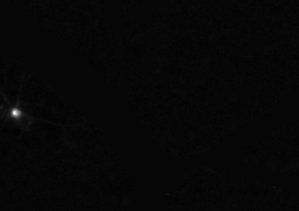
\includegraphics[width=.9\linewidth]{frame_2.png}
      \caption*{\footnotesize A) Clean neuron source frame.}
      \label{fig:frame1}
    \end{minipage}%
    \begin{minipage}{.33\textwidth}
      \centering
      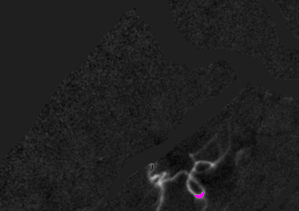
\includegraphics[width=.9\linewidth]{frame_3.png}
      \caption*{\footnotesize B) Background structure. }
      \label{fig:frame2}
    \end{minipage}
    \begin{minipage}{.33\textwidth}
      \centering
      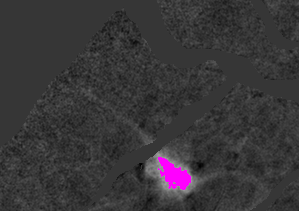
\includegraphics[width=.9\linewidth]{frame_4.png}
      \caption*{\footnotesize C) Large neuron. }
      \label{fig:frame3}
    \end{minipage}
    \caption{\footnotesize Examples of frame data. (A) contains a clean neuron source frame. (B) contains background structure in the form of blood vessels. The FWHM peak region is colored magenta. (C) contains an unknown structure which is likely a neuron. Here the peak region is much larger. }
\end{figure}

A set of twelve features were extracted for each image frame.
A frame is a \num{500} by \num{500} pixel monochromatic matrix containing the average IC over the segemented field of view. 
Image frame values background noise fluctuates on the order of \num{+-3} but contains sharp peak values as high as \num{100} in intensity.

A single peak region was identified in each image using the full-width half maximum.
All pixels above half the maximum value were considered, and a flood-fill algorithm was used to find the largest connected region, hereafter referred to as the peak region.

Several features are derived directly from the peak region.
The \emph{peak region size} is the number of pixels in the peak region, and corresponds roughly to the area of the peak region.
The \emph{peak region perimeter} is the number of pixels on the exterior of the peak region, and corresponds roughly to the perimeter of the peak region.
An approximate measure of \emph{roundness} was obtained by computing the ratio of the peak region size and perimeter, $\text{roundness} = 4\pi \sfrac{\text{area}}{\text{perimeter}^2}$, 
where a roundness of one corresponds roughly to a perfect circle.
The peak region \emph{skew} was obtained by computing the $xy$-correlation between the square subsection of the image of twenty-one pixel side length centered at the peak region center.
The \emph{peak} value of the peak region was extracted, as well as the peak region \emph{mean} and \emph{standard deviation}.

A subimage of twenty-four pixel side length was extracted about the peak region center and used to compute additional features, among them the mean and standard deviation of the subimage.
A measure of \emph{contrast} and \emph{directionality} was obtained using the Tamura definition~\cite{Tamura1978}.
Contrast is a measure of image sharpness, and was calculated using

$$
F_\text{con} = \frac{\sigma}{\alpha_4^z} \quad \text{with} \quad \alpha_4 = \frac{\mu_4}{\sigma^4}
$$

\noindent
where $\mu_4 = \frac{1}{nm} \sum_{i=1}^n \sum_{j=1}^m (IC(i,j)-\mu)^4$
is the fourth moment about the mean $\mu$, $z$ is \num{0.25} from experiment, and $\sigma^2$ is the variance of the image values.

Directionality was computed using the approximate horizontal and vertical derivatives from convolution with the following $3\times3$ matrices, respectively $\Delta_V$ and $\Delta_H$:

$$
\begin{bmatrix}
-1 & 0 & 1 \\ -1 & 0 & 1 \\ -1 & 0 & 1
\end{bmatrix} \qquad
\begin{bmatrix}
-1 & -1 & -1 \\
0 & 0 & 0 \\
1 & 1 & 1
\end{bmatrix}
$$

\noindent
and then computing $\theta = \frac{\pi}{2} + \tan^{-1}\frac{\Delta_V(i,j)}{\Delta_H(i,j)}$ for each pixel in the image.
These values were discretized into a sixteen bin histogram.

Some peak images are very close to their segmented image borders. For these images it is not possible to extract the subimage.
The corresponding features were imputed using the method of iterated singular value decomposition of rank \num{10}.

\subsection{Trace Features}

Calcium activity for a perfectly recorded neuron takes the form of temporally sparse spikes that start with a fast jump followed by exponential decay. Spike sparsity and exponential decay constants vary between neurons~\cite{Mukamel2009}. 
An example trace is shown in \cref{fig:trace}.

For each trace a \emph{high threshold} and \emph{low threshold} were calculated where the \emph{CDF} used is \todo{\num{0.97}} and \todo{\num{0.03}} respectively. In addition, every time the trace crosses the high threshold and low threshold line, a high crossing and low crossing event is detected. These events can be described by a \emph{rise time}, \emph{fall time} and \emph{pick value}. Average and variance of these three variables were also computed. The \emph{ratio of mean pick value to threshold value} of high or low crossings were also extraced.

The sparsity of neural activity has been previously shown to be a good indicator~\cite{Kim2011}. Average and variance of \emph{crossing event intervals} for high and low crossings were taken where each interval is the time distance between two picks of the crossing events.  The ratio of \emph{total crossing duration} to the total time were calculated for each family separately and taken as a sparsity measure. Neurons are expected to have primarily high crossing events. The \emph{number of high crossing events}, \emph{number of low crossing events} and the ratio of these two were also included. The final trace feature vector includes \num{30} indices.

% \begin{figure}[h]
%     \centering

%     \begin{minipage}{1\textwidth}
%       \centering
%       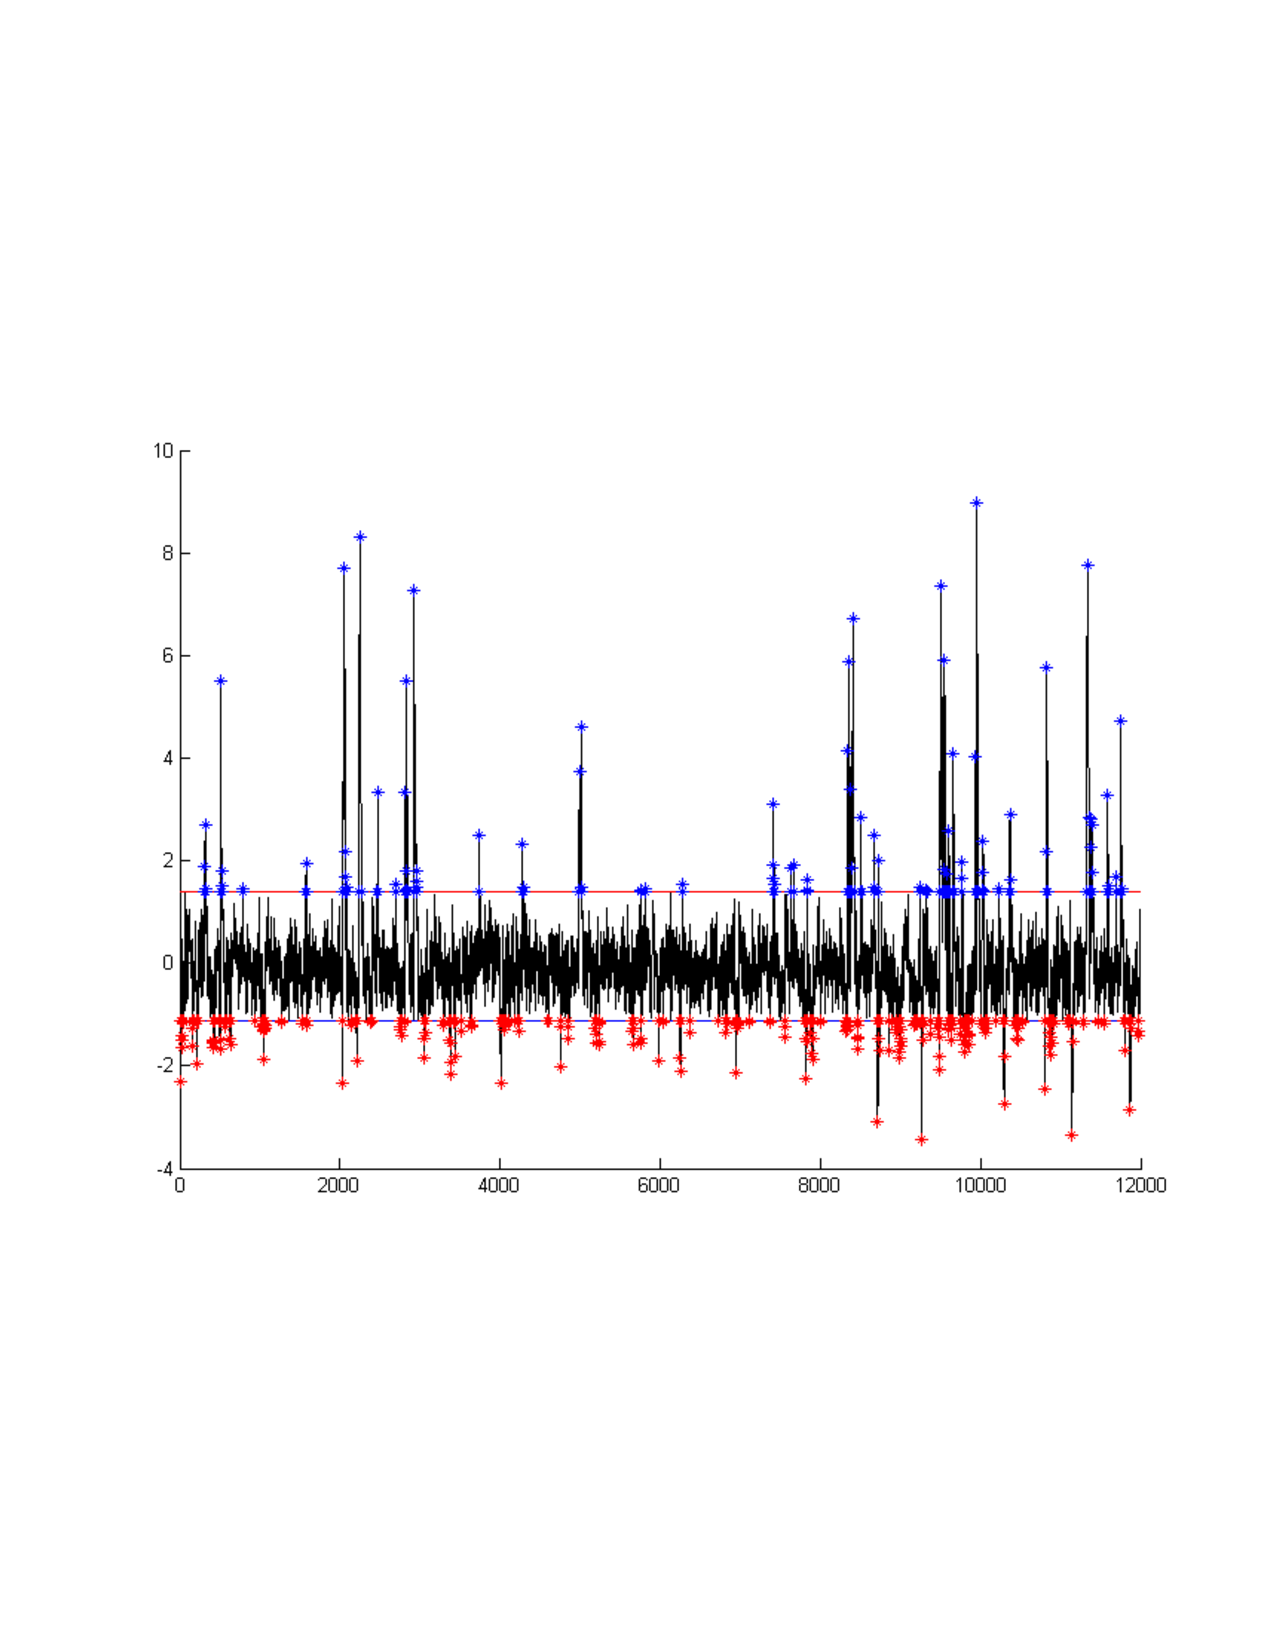
\includegraphics[width=0.5\linewidth]{trace.pdf}
%       \caption{\footnotesize Example neuron Calcium trace. \textcolor{blue}{blue *} indicates start, pick and end of high crossing events and \textcolor{red}{red *} indicates the same time points in low crossing events }
%       \label{fig:trace}
%     \end{minipage}
  
% \end{figure}

\section{Analysis}

The objective of this analysis is to identify clusters within the calcium imaging dataset which correspond to neurons and background structure, respectively. During the process it may be possible to further identify subclusters which correspond to different types of neurons or types of background structure.

Hierarchical clustering possesses several advantages over partitional clustering for this problem.
First, most of the features in the dataset are continuous and poorly separated, making it difficult to a partitional algorithm such as $k$-means to accurately divide it by a valid hard boundary. 
Secondly, hierarchical clustering produces dendrograms, which contain a full range of clusters, allowing for the appropriate cutoff point to be chosen by a statistician via inspection. 
\todo{Can you think of a third reason?}

The dataset was subjected to several forms of hierarchical clustering in an effort to identify suitable neuronal clusters and identify the most important features. 
All analysis was done using a data matrix in which each feature vector was de-meaned and divided by its standard deviation.
A final round of analysis was performed to validate the obtained clusters against a second withheld dataset.

\subsection{Full Hierarchical Clustering}

Agglomerative clustering using complete linking and Euclidean distance was conducted and the results are shown in \cref{fig:fullhierarchical}.
The resulting dendrogram contains several well-separated clusters containing almost entirely neurons or background noise, with few samples from the opposite class.

\begin{figure}[h]
    \centering

    \begin{minipage}{0.55\textwidth}
      \centering
      \includegraphics[width=0.9\textwidth]{/home/tim/Documents/Schoolwork/win2015stats306b/code/heatmap.pdf}
    \end{minipage}
    \begin{minipage}{0.4\textwidth}
      \centering
      \scriptsize
      \begin{tabular}{cSS}
        \toprule
        Cluster & {Size} & {Percent Neuronal Content} \\
        \midrule
        cluster 1 & 2500 & 95.0 \\
        cluster 2 & 1500 & 95.0 \\
        cluster 3 & 2500 &  5.0 \\
        cluster 4 & 2500 &  3.0 \\
        \bottomrule
      \end{tabular}
    \end{minipage}
    \caption{\footnotesize Full hierarchical clustering and associated cluster statistics. \todo{Re-run with correctly labelled trace features and color-code.}}
    \label{fig:fullhierarchical}
\end{figure}

\todo{Proceed with an investigation of the cluster contents. Are the neuronal clusters different? Are the background clusters different?}
\todo{Include scatter plots with important features, etc.}

\subsection{Principle Component Analysis}

Further insight into the relative importance of features in clustering was obtained by investigating the principle components.
A principle component analysis of the data matrix revealed that \todo{XX\%} of the variation in the data is captured in the first two components.
The first component variest most widely in \todo{blah blah.}
The second principle component variest captures additional variatio in \todo{blah blah}.

\begin{figure}[h]
    \centering

    \begin{minipage}{0.4\textwidth}
      \centering
      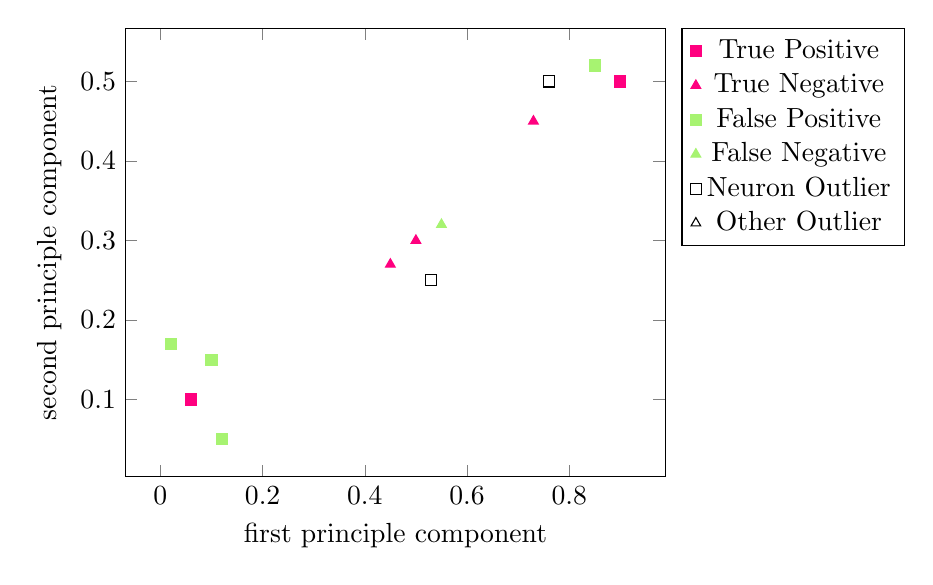
\begin{tikzpicture}
        \begin{axis}[%
            scatter/classes={%
                sb={mark=square*,   color3},%
                tb={mark=triangle*, color3},%
                sr={mark=square*,   color2},%
                tr={mark=triangle*, color2},%
                sk={mark=square,    draw=black},%
                tk={mark=triangle,  draw=black}%
                },
            legend style={at={(1.03,1.0)}, anchor=north west},
            xlabel=first principle component,
            ylabel=second principle component
            ]
            
            \addplot[scatter,only marks, scatter src=explicit symbolic] table[meta=label] {
                        x     y      label
                        0.1   0.15   sr
                        0.45  0.27   tb
                        0.02  0.17   sr
                        0.06  0.1    sb
                        0.9   0.5    sb
                        0.5   0.3    tb
                        0.85  0.52   sr
                        0.12  0.05   sr
                        0.73  0.45   tb
                        0.53  0.25   sk
                        0.76  0.5    sk
                        0.55  0.32   tr
            };
            \legend{True Positive, True Negative, False Positive, False Negative, Neuron Outlier, Other Outlier};
        \end{axis}
      \end{tikzpicture}
    \end{minipage}
    \caption{\footnotesize Scatter plot of clusters. \todo{Load correct data from csv} }
    \label{fig:fullhierarchical}
\end{figure}

\todo{Include some more discussion of results.}

\subsection{Sparse Hierarchical Clustering}

\todo{Wherein we use sparcl to perform sparse clustering}
\todo{This section needs an image (probably a repeat of what we have above - a dendrogram and a cluster table)}.
\todo{Finish it up with a discussion of what it is we discovered.}

\subsection{Group Validation}

\todo{Wherein we compare the clusters obtained in dataset A to those found in dataset B}
\todo{Use the metric of in-group proportion to compute the centroid for groups in the training set, and then assign objects in set 2 to the closest centroid. The in-group proportion is the proportion of observations in the second group whose nearest neighbor is also in that group. I hope that there is an R package for this.}
\todo{One can compute a p-value for this as well.}
\todo{Should include an image of the second group's dendrogram}.

\section{Conclusions and Future Work}

\todo{Recap what was done}
\todo{Did we successfully identify clusters?}
\todo{Did we discover any sub-clusters within the neuron group or structure group?}
\todo{Did we successfully identify important features?}
\todo{How did group validation go?}

\todo{Some ideas for future work.}

% \newpage

\printbibliography

\end{document}